\documentclass{standalone}
\usepackage{tikz}
\usetikzlibrary{patterns, positioning}

\begin{document}
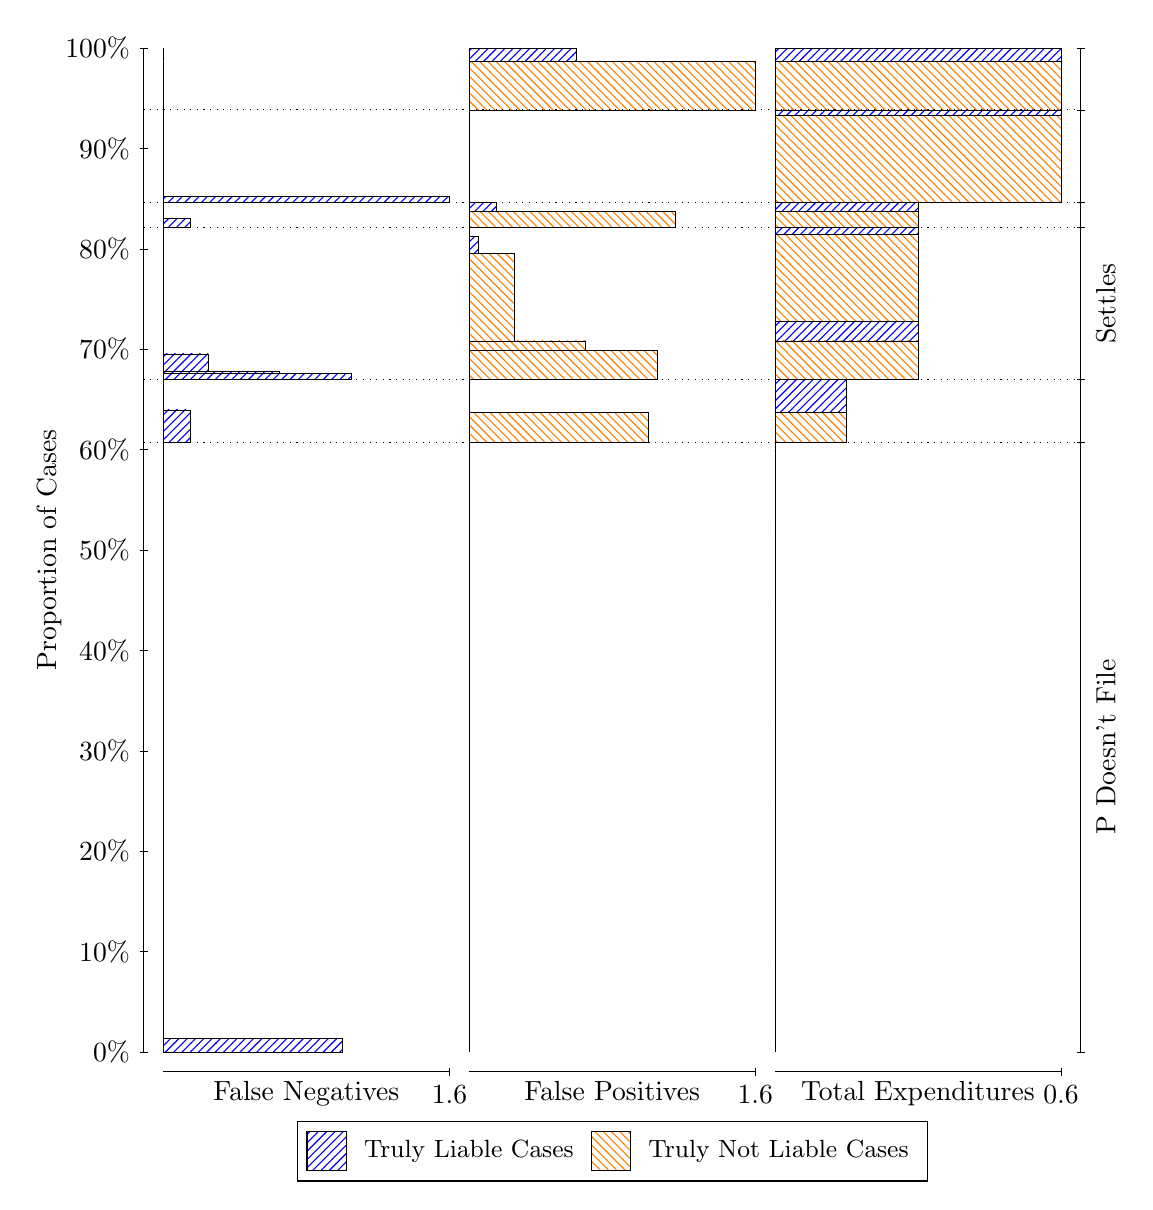
\begin{tikzpicture}
\draw[black, very thin] (1.5,1.75) -- (1.5,14.5);
\node[rotate=90, anchor=center] at (0.3, 8.125) {Proportion of Cases};
\draw[black, very thin] (1.45,1.75) -- (1.55,1.75);
\node[anchor=east] at (1.45, 1.75) {0\%};
\draw[black, very thin] (1.45,3.025) -- (1.55,3.025);
\node[anchor=east] at (1.45, 3.025) {10\%};
\draw[black, very thin] (1.45,4.3) -- (1.55,4.3);
\node[anchor=east] at (1.45, 4.3) {20\%};
\draw[black, very thin] (1.45,5.575) -- (1.55,5.575);
\node[anchor=east] at (1.45, 5.575) {30\%};
\draw[black, very thin] (1.45,6.85) -- (1.55,6.85);
\node[anchor=east] at (1.45, 6.85) {40\%};
\draw[black, very thin] (1.45,8.125) -- (1.55,8.125);
\node[anchor=east] at (1.45, 8.125) {50\%};
\draw[black, very thin] (1.45,9.4) -- (1.55,9.4);
\node[anchor=east] at (1.45, 9.4) {60\%};
\draw[black, very thin] (1.45,10.675) -- (1.55,10.675);
\node[anchor=east] at (1.45, 10.675) {70\%};
\draw[black, very thin] (1.45,11.95) -- (1.55,11.95);
\node[anchor=east] at (1.45, 11.95) {80\%};
\draw[black, very thin] (1.45,13.225) -- (1.55,13.225);
\node[anchor=east] at (1.45, 13.225) {90\%};
\draw[black, very thin] (1.45,14.5) -- (1.55,14.5);
\node[anchor=east] at (1.45, 14.5) {100\%};

\draw[black, very thin] (13.4,1.75) -- (13.4,14.5);
\draw[black, very thin] (13.35,1.75) -- (13.45,1.75);
\node[anchor=west] at (13.35, 1.75) {};
\draw[black, very thin] (13.35,9.4955) -- (13.45,9.4955);
\node[anchor=west] at (13.35, 9.4955) {};
\draw[black, very thin] (13.35,10.287) -- (13.45,10.287);
\node[anchor=west] at (13.35, 10.287) {};
\draw[black, very thin] (13.35,12.219) -- (13.45,12.219);
\node[anchor=west] at (13.35, 12.219) {};
\draw[black, very thin] (13.35,12.543) -- (13.45,12.543);
\node[anchor=west] at (13.35, 12.543) {};
\draw[black, very thin] (13.35,13.715) -- (13.45,13.715);
\node[anchor=west] at (13.35, 13.715) {};
\draw[black, very thin] (13.35,14.5) -- (13.45,14.5);
\node[anchor=west] at (13.35, 14.5) {};

\draw[black, very thin, pattern color=blue, pattern=north east lines] (1.75,1.75) rectangle (4.0208,1.9249);
\draw[black, very thin, pattern color=orange, pattern=north west lines] (1.75,1.9249) rectangle (1.75,9.4955);
\draw[black, very thin, pattern color=blue, pattern=north east lines] (1.75,9.4955) rectangle (2.0906,9.9055);
\draw[black, very thin, pattern color=orange, pattern=north west lines] (1.75,9.9055) rectangle (1.75,10.287);
\draw[black, very thin, pattern color=blue, pattern=north east lines] (1.75,10.287) rectangle (4.1344,10.368);
\draw[black, very thin, pattern color=blue, pattern=north east lines] (1.75,10.368) rectangle (3.226,10.398);
\draw[black, very thin, pattern color=blue, pattern=north east lines] (1.75,10.398) rectangle (2.3177,10.616);
\draw[black, very thin, pattern color=orange, pattern=north west lines] (1.75,10.616) rectangle (1.75,12.219);
\draw[black, very thin, pattern color=blue, pattern=north east lines] (1.75,12.219) rectangle (2.0906,12.339);
\draw[black, very thin, pattern color=orange, pattern=north west lines] (1.75,12.339) rectangle (1.75,12.543);
\draw[black, very thin, pattern color=blue, pattern=north east lines] (1.75,12.543) rectangle (5.3833,12.611);
\draw[black, very thin, pattern color=orange, pattern=north west lines] (1.75,12.611) rectangle (1.75,13.715);
\draw[black, very thin, pattern color=orange, pattern=north west lines] (1.75,13.715) rectangle (1.75,14.327);
\draw[black, very thin, pattern color=blue, pattern=north east lines] (1.75,14.327) rectangle (1.75,14.5);
\draw[black, very thin, pattern color=orange, pattern=north west lines] (5.6333,1.75) rectangle (5.6333,9.3206);
\draw[black, very thin, pattern color=blue, pattern=north east lines] (5.6333,9.3206) rectangle (5.6333,9.4955);
\draw[black, very thin, pattern color=orange, pattern=north west lines] (5.6333,9.4955) rectangle (7.9042,9.8769);
\draw[black, very thin, pattern color=blue, pattern=north east lines] (5.6333,9.8769) rectangle (5.6333,10.287);
\draw[black, very thin, pattern color=orange, pattern=north west lines] (5.6333,10.287) rectangle (8.0177,10.661);
\draw[black, very thin, pattern color=orange, pattern=north west lines] (5.6333,10.661) rectangle (7.1094,10.78);
\draw[black, very thin, pattern color=orange, pattern=north west lines] (5.6333,10.78) rectangle (6.201,11.89);
\draw[black, very thin, pattern color=blue, pattern=north east lines] (5.6333,11.89) rectangle (5.7469,12.109);
\draw[black, very thin, pattern color=blue, pattern=north east lines] (5.6333,12.109) rectangle (5.6333,12.219);
\draw[black, very thin, pattern color=orange, pattern=north west lines] (5.6333,12.219) rectangle (8.2448,12.423);
\draw[black, very thin, pattern color=blue, pattern=north east lines] (5.6333,12.423) rectangle (5.974,12.543);
\draw[black, very thin, pattern color=orange, pattern=north west lines] (5.6333,12.543) rectangle (5.6333,13.647);
\draw[black, very thin, pattern color=blue, pattern=north east lines] (5.6333,13.647) rectangle (5.6333,13.715);
\draw[black, very thin, pattern color=orange, pattern=north west lines] (5.6333,13.715) rectangle (9.2667,14.327);
\draw[black, very thin, pattern color=blue, pattern=north east lines] (5.6333,14.327) rectangle (6.9958,14.5);
\draw[black, very thin, pattern color=orange, pattern=north west lines] (9.5167,1.75) rectangle (9.5167,9.3206);
\draw[black, very thin, pattern color=blue, pattern=north east lines] (9.5167,9.3206) rectangle (9.5167,9.4955);
\draw[black, very thin, pattern color=orange, pattern=north west lines] (9.5167,9.4955) rectangle (10.425,9.8769);
\draw[black, very thin, pattern color=blue, pattern=north east lines] (9.5167,9.8769) rectangle (10.425,10.287);
\draw[black, very thin, pattern color=orange, pattern=north west lines] (9.5167,10.287) rectangle (11.333,10.78);
\draw[black, very thin, pattern color=blue, pattern=north east lines] (9.5167,10.78) rectangle (11.333,11.028);
\draw[black, very thin, pattern color=orange, pattern=north west lines] (9.5167,11.028) rectangle (11.333,12.138);
\draw[black, very thin, pattern color=blue, pattern=north east lines] (9.5167,12.138) rectangle (11.333,12.219);
\draw[black, very thin, pattern color=orange, pattern=north west lines] (9.5167,12.219) rectangle (11.333,12.423);
\draw[black, very thin, pattern color=blue, pattern=north east lines] (9.5167,12.423) rectangle (11.333,12.543);
\draw[black, very thin, pattern color=orange, pattern=north west lines] (9.5167,12.543) rectangle (13.15,13.647);
\draw[black, very thin, pattern color=blue, pattern=north east lines] (9.5167,13.647) rectangle (13.15,13.715);
\draw[black, very thin, pattern color=orange, pattern=north west lines] (9.5167,13.715) rectangle (13.15,14.327);
\draw[black, very thin, pattern color=blue, pattern=north east lines] (9.5167,14.327) rectangle (13.15,14.5);
\draw[black, dotted] (1.5,9.4955) -- (13.4,9.4955);
\draw[black, dotted] (1.5,10.287) -- (13.4,10.287);
\draw[black, dotted] (1.5,12.219) -- (13.4,12.219);
\draw[black, dotted] (1.5,12.543) -- (13.4,12.543);
\draw[black, dotted] (1.5,13.715) -- (13.4,13.715);
\draw[black, very thin] (1.75,1.5) -- (5.3833,1.5);
\node[anchor=north] at (3.5667, 1.5) {False Negatives};
\draw[black, very thin] (5.3833,1.45) -- (5.3833,1.55);
\node[anchor=north] at (5.3833, 1.45) {1.6};

\draw[black, very thin] (5.6333,1.5) -- (9.2667,1.5);
\node[anchor=north] at (7.45, 1.5) {False Positives};
\draw[black, very thin] (9.2667,1.45) -- (9.2667,1.55);
\node[anchor=north] at (9.2667, 1.45) {1.6};

\draw[black, very thin] (9.5167,1.5) -- (13.15,1.5);
\node[anchor=north] at (11.333, 1.5) {Total Expenditures};
\draw[black, very thin] (13.15,1.45) -- (13.15,1.55);
\node[anchor=north] at (13.15, 1.45) {0.6};

\node[black, centered, rotate=90] at (13.72, 5.6227) {P Doesn't File};

\node[black, centered, rotate=90] at (13.72, 11.253) {Settles};




\draw (7.449999999999999,1.5) node[draw=none] (baseCoordinate) {};
\begin{scope}[align=center]
        \matrix[scale=0.5, draw=black, below=0.5cm of baseCoordinate, nodes={draw}, column sep=0.1cm]{
            \node[rectangle, draw, minimum width=0.5cm, minimum height=0.5cm, pattern=north east lines, pattern color=blue] {}; &
            \node[draw=none, font=\small] (B) {Truly Liable Cases}; &
            \node[rectangle, draw, minimum width=0.5cm, minimum height=0.5cm, pattern=north west lines, pattern color=orange] {}; &
            \node[draw=none, font=\small] (B) {Truly Not Liable Cases}; \\
            };
\end{scope}

\end{tikzpicture}
\end{document}